\documentclass{standalone}
\usepackage{tikz,ctex}
\usepackage{tikz-3dplot} % 2-1
\usepackage{unicode-math} % 2-5,4-1,4-2
\setmathfont{Fira Math Regular}
\setmainfont{Fira Sans}
\definecolor{background}{RGB}{239, 239, 239} % 4-5,6-2,6-5
\begin{document}
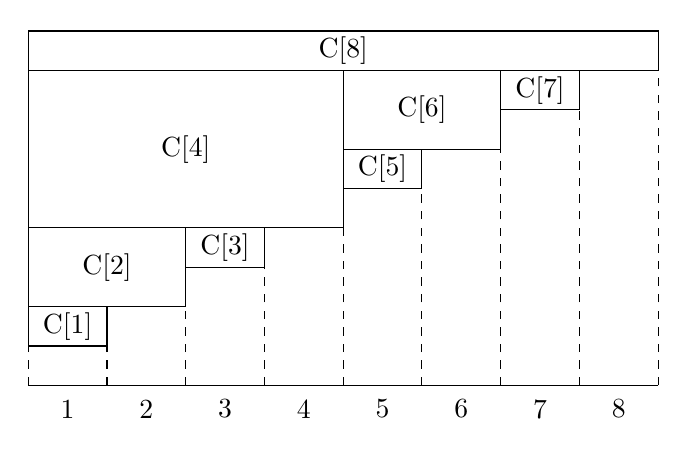
\begin{tikzpicture}
\foreach \x/\y/\a/\b[count=\i] in {1/1.5/2/2, 1/2/3/3, 3/2.5/4/3, 1/3/5/5, 5/3.5/6/4, 5/4/7/5, 7/4.5/8/5, 1/5/9/5.5}{
    \draw (\x,\y) rectangle (\a,\b) node[midway]{C[\i]};}
\draw (1,1)--(9,1);
\foreach \x in {1,...,8}{
    \draw[dashed] (\x,1)--(\x,1+.5*\x);
    \node at (\x+.5,.7){\x};}
\draw[dashed] (9,1)--(9,5.5);
\end{tikzpicture}
\end{document}